



\section{Problem Setup}
\label{sec:problem}
Online action anticipation and detection share a similar goal of predicting actions in untrimmed video sequences. In the former, we aim to forecast actions after a time gap $\tau$, as defined in~\cite{ek100}, while in the latter, we predict the action under $\tau=0$.
Both tasks require classifying actions without access to future information during inference.
We represent the input video as 
$ \mathbf{V} = \{ v_t \}_{t = -T + 1}^{0} $,
and our objective is to predict the action category $\hat{y}_{\tau} \in \{ 0, 1, 2, \dots, C \}$ occurs after a specified time gap $\tau$ in the future. Here, $C$ represents the total number of action categories, and label $ 0 $ denotes the background category.



\section{Memory-and-Anticipation Transformer}
\label{sec:approach}
We now describe Memory-and-Anticipation Transformer (MAT) model architecture, as illustrated in Fig~\ref{fig:framework}. It processes the memory cached in runtime to predict current or future actions. We adopt the \emph{encoder-decoder} architecture to implement the model. The \emph{Progressive Memory Encoder} is proposed to improve the quality of compressing long-term memory and enhancing short-term memory, which has a fundamental impact on anticipation and detection. MAT also employs our presented key component \emph{Memory-Anticipation Circular Decoder} that generates the latent anticipation feature and conducts interaction between memory and anticipation in an iterative loop.
We now introduce each model component in detail, followed by the training, online inference, and implementation details.

\subsection{Progressive Memory Encoder}

We use video feature $\mathbf{F} = \{ f_t \}_{t = -T + 1}^{0} \in \mathbb{R}^{T \times D}$ generated by a pretrained feature extractor as the input to our model, where $D$ and $T$ are the dimension and length of the feature sequence, respectively. 
To better handle the long memory, following~\cite{lstr}, we divide the feature sequence into two consecutive memories. The first is the short-term memory that stores only a handful of recently occurred frames. It stores the feature vectors as $ \mathbf{M}_S = \{ f_t \}_{t = -m_S + 1}^{0}$, where $ m_S $ denotes the length. The other, named long-term memory, contains the feature that is far away from the current time, which is defined as $\mathbf{M}_L = \{ f_t \}_{t = -T + 1}^{-m_S} $. We set $ m_L $ to be the length of the long-term memory, which is much longer than the short-term memory.

In practice, \emph{Progressive Memory Encoder} progressively encodes long- and short-term memories. It first compresses the long-term memory to an abstract representation and injects them into the short-term memory. 
Differing with previous works~\cite{lstr, testra} that separately tackle the long- and short-term memories by one long-term encoder and one short-term decoder, we integrate these two works into a single encoder architecture.
It is due to our encoded short-term memory being served for decoders and not as the final output. In our experiments, we observe that the design of the memory encoder is crucial for model performance. Therefore, different with~\cite{lstr, testra}, we introduce a novel long-term memory compression method to improve the quality of memory encoding.

\textbf{Segment-based Long-term Memory Compression.}
LSTR~\cite{lstr} adopts a two-stage compression technique to project the long-term memory to a fixed-length latent embedding. It implements a function similar to the bottleneck layer~\cite{resnet}. 
Long-term memory, however, represents a long token sequence that often carries much noise.
It is problematic to generate attention weights while cross-attention queries too many tokens with mixed noise. 
We propose \emph{Segment-based Long-term Memory Compression} to alleviate the issue, as shown in Fig~\ref{fig:encoder}.
Concretely, we first divide $\mathbf{M}_{L}$ into $N_s$ non-overlapping memory segments  
$ \mathbf{S} = \{ \mathbf{s}_{i}\}^{N_s}_{i=1} $ of length $\frac{m_L}{N_s}$.
We then employ $N_L$ learnable tokens $ \mathbf{Q}_{L} \in \mathbb{R}^{ N_L \times D }$ as the long-term memory queries and a weight-shared transformer decoder block to query each segment. 
$\mathbf{S}$ will be transformed to $N_s$ segment-level abstract feature $\mathbf{F} =\{ \mathbf{f}_{i}\}^{N_s}_{i=1}$, where $\mathbf{f}_{i} \in \mathbb{R}^{ N_L \times D }$. We average pool each $\mathbf{f}_{i}$ to one vector $\mathbb{R}^{ D }$ and concatenate them to form the long-term compressed segmented memory $\mathbf{M}_L^s \in \mathbb{R}^{ N_s \times D }$.
At last, we feed them into two transformer encoder blocks to obtain the final compressed long-term memory $ \mathbf{\widehat{M}}_L \in \mathbb{R}^{N_s \times D} $.  
 


\textbf{Short-term Memory Enhancement.}
As short-term memory $ \mathbf{M}_S = \{ f_t \}_{t = -m_S + 1}^{0} $ contains crucial trends for accurately predicting the current or upcoming activities, we leverage short-term memory as the query to retrieve relevant context from the compressed long-term memory.
As illustrated in Fig~\ref{fig:framework}, we employ a transformer causal decoder block to aggregate compressed long-term memory $\mathbf{\widehat{M}}_L$ into short-term memory. The enhanced short-term memory $\mathbf{\widehat{M}}_S$ is then used to identify actions at each timestep, constituting a sequence of previously occurring actions and predicting future states and actions. We use frame-level action labels to supervise the dense classification task, encouraging the model to produce a clear sequence of historical behavior.



\subsection{Memory-Anticipation Circular Decoder}
\label{decoder}
To implement our key idea that considers the co-reaction between anticipation and memory, we carefully design \emph{Memory-Anticipation Circular Decoder} that circularly performs interaction between them. It first generates the latent anticipation that is a prerequisite for memory-anticipation interaction. Then, \emph{Conditional Circular Interaction} will generate new memories and anticipation conditioned on old ones iteratively. Finally, a weight-shared classification head will supervise the generated memories and anticipation.


\textbf{Latent Anticipation Generation.}
Initially, we do not have an anticipation state. Therefore, we must first generate a latent anticipation feature, \ie, a future representation containing abstract information derived from known memory. 
Given the compressed long-term memory $\mathbf{\widehat{M}}_L$ and short-term memory $\mathbf{\widehat{M}}_S$, we first concatenate them to form the entire memory $\mathbf{M}_E = [\mathbf{\widehat{M}}_L, \mathbf{\widehat{M}}_S]  $, where $[\cdot,\cdot]$ is the concatenating operation along the temporal dimension. 
Then, we use $N_F$ future queries $\mathbf{Q}_F \in \mathbb{R}^{ N_F \times D }$ and a transformer decoder block to query $\mathbf{M}_E$. The updated future queries are represented as the latent anticipation features $\mathbf{F}_{A}\in \mathbb{R}^{ N_F \times D}$ at the current state. We use future information, \eg, future video features and future action labels, to supervise $\mathbf{F}_{A}$. In practice, we use information from the next $T_F$ seconds. Since $\mathbf{F}_{A}$ is only used to describe the latent future states, too large future embeddings may overfit the anticipation representation. We set $N_F$ to be smaller than the length of the used future information sequence. Then we use bilinear interpolation to upsample it to align for point-to-point supervision. Note that although we use future information here, this does not lead to an information leak. The model will generate preliminary anticipation in the inference phase and not use future labels or features.

\begin{figure}
    \centering
    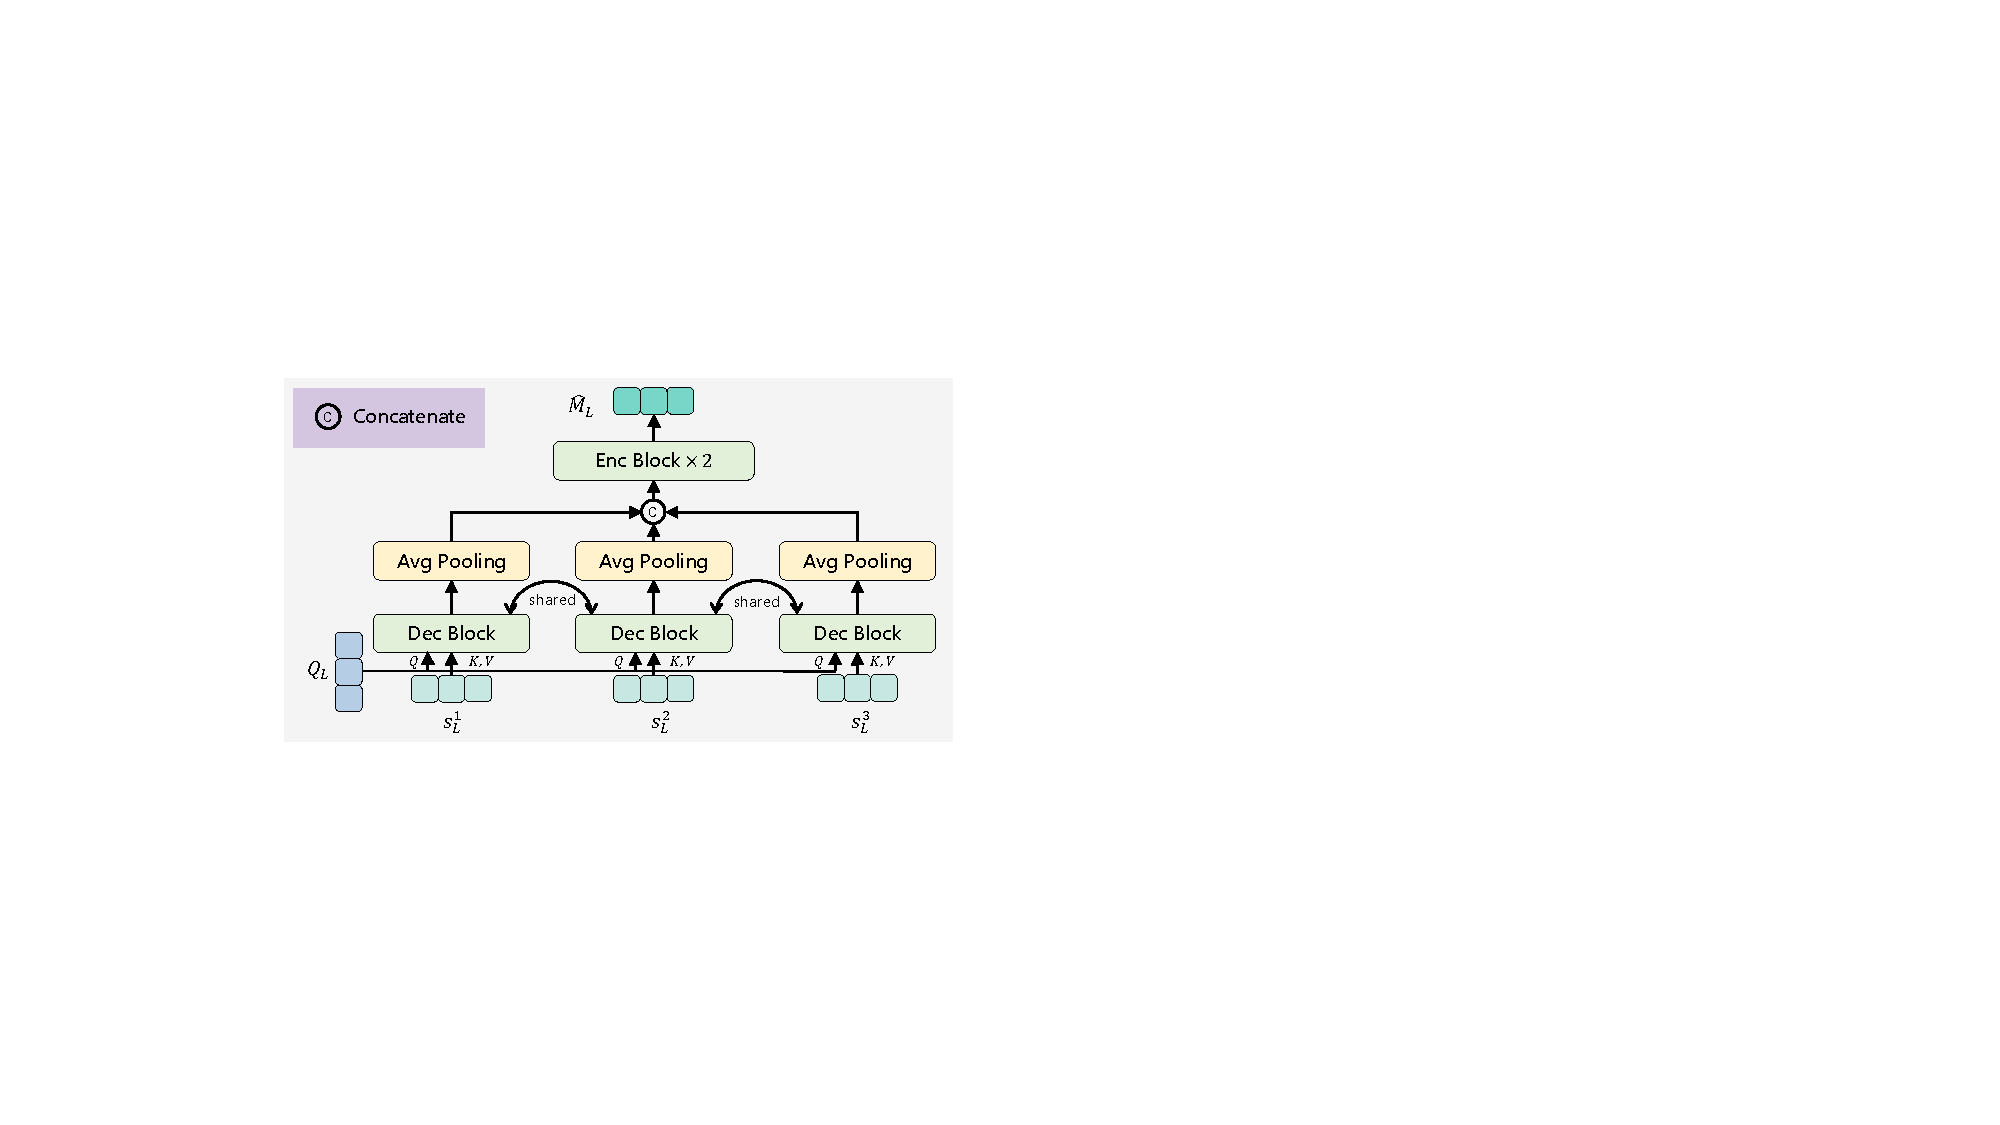
\includegraphics[width=0.48\textwidth]{images/Encoder.pdf}
    \caption{\textbf{Segment-based Long-term Memory Compression.} 
    For example, given $ m_L = 9, N_s = 3$, the process is shown above. We can finally obtain compressed features $ \widehat{M}_L $ of length 3.}
    \label{fig:encoder}
\end{figure}







\textbf{Conditional Circular Interaction.}
So far, we have generated long-term memory $\mathbf{\widehat{M}}_L$, short-term memory $\mathbf{\widehat{M}}_S$ and latent anticipation features $\mathbf{F}_A$. The memories, however, are limited to the past and can not go beyond history. 
We now describe how \emph{Conditional Circular Interaction} works.
For brevity, we detail how memory and anticipation interact with each other one time.


As shown in Fig~\ref{cci}, we first concatenate $\mathbf{\widehat{M}}_L$, $\mathbf{\widehat{M}}_S$ and $\mathbf{F}_A$ to form the entire feature $\mathbf{F}_E = [\mathbf{\widehat{M}}_L, \mathbf{\widehat{M}}_S, \mathbf{F}_A]$. 
Then, $\mathbf{F}_E$ and $\mathbf{\widehat{M}}_S$ are feed into a transformer decoder block:
\begin{equation}
    \begin{aligned}
        \mathbf{\widehat{M}}_S^{\prime} = \text{CrossAttn}(\mathbf{\widehat{M}}_S,\mathbf{F}_E,\mathbf{F}_E),
    \end{aligned}
\end{equation}
where $\text{CrossAttn}(Q,K,V)$ is the cross-attention layer in the transformer decoder block. The updated short-term memory is represented as $\mathbf{\widehat{M}}_S^{\prime}$. Since $\mathbf{F}_E$ contains memories and anticipation, $\mathbf{\widehat{M}}_S$ as a query condition dynamically extracts new semantics mixed with memories and anticipation from three representations.  Next, we re-concatenate $\mathbf{\widehat{M}}_L$, $\mathbf{\widehat{M}}_S^{\prime}$ and $\mathbf{F}_A$ to generate the new entire feature $\mathbf{F}_E^{\prime} = [\mathbf{\widehat{M}}_L, \mathbf{\widehat{M}}_S^{\prime}, \mathbf{F}_A]$. Another transformer decoder block is used to query $\mathbf{F}_E^{\prime}$, with $\mathbf{F}_A$ as the query condition:
\begin{equation}
    \begin{aligned}
        \mathbf{\mathbf{F}}_A^{\prime} = \text{CrossAttn}(\mathbf{F}_A,\mathbf{F}_E^{\prime},\mathbf{F}_E^{\prime}),
    \end{aligned}
\end{equation}
where $\mathbf{F}_A^{\prime}$ is the resulting anticipation features.
After that, $\mathbf{F}_A^{\prime}$ is injected with the higher-order inferred semantics brought about by the interaction between memory and anticipation.

In the interaction process, the generated $\mathbf{\widehat{M}}_S^{\prime}$ is both supervised like the above initial anticipation features. It should be noted that different from generating latent initial anticipation through fewer future queries, we find that using a new group of future queries $\mathbf{Q}_F^{\prime} \in \mathbb{R}^{ N_F^{\prime} \times D }$ strictly aligned future information sequences of $T_F$ seconds in the first interaction process to replace the $\mathbf{F}_A$ with $\mathbf{Q}_F^{\prime}$, bring performance improvement. Thus, we point-to-point supervise the anticipation $\mathbf{F}_A^{\prime}$ generated by each interaction process. Meanwhile, this design is more natural to output the corresponding token according to the anticipation gap time.
We circularly perform the interaction process $N_t$ times until saturation. The yielded  $\mathbf{\widehat{M}}_S^{\prime}$ and $\mathbf{F}_A^{\prime}$ in one interaction process become the new $\mathbf{\widehat{M}}_S$ and $\mathbf{F}_A$ and are passed to the next interaction process. 

\begin{figure}
    \centering
    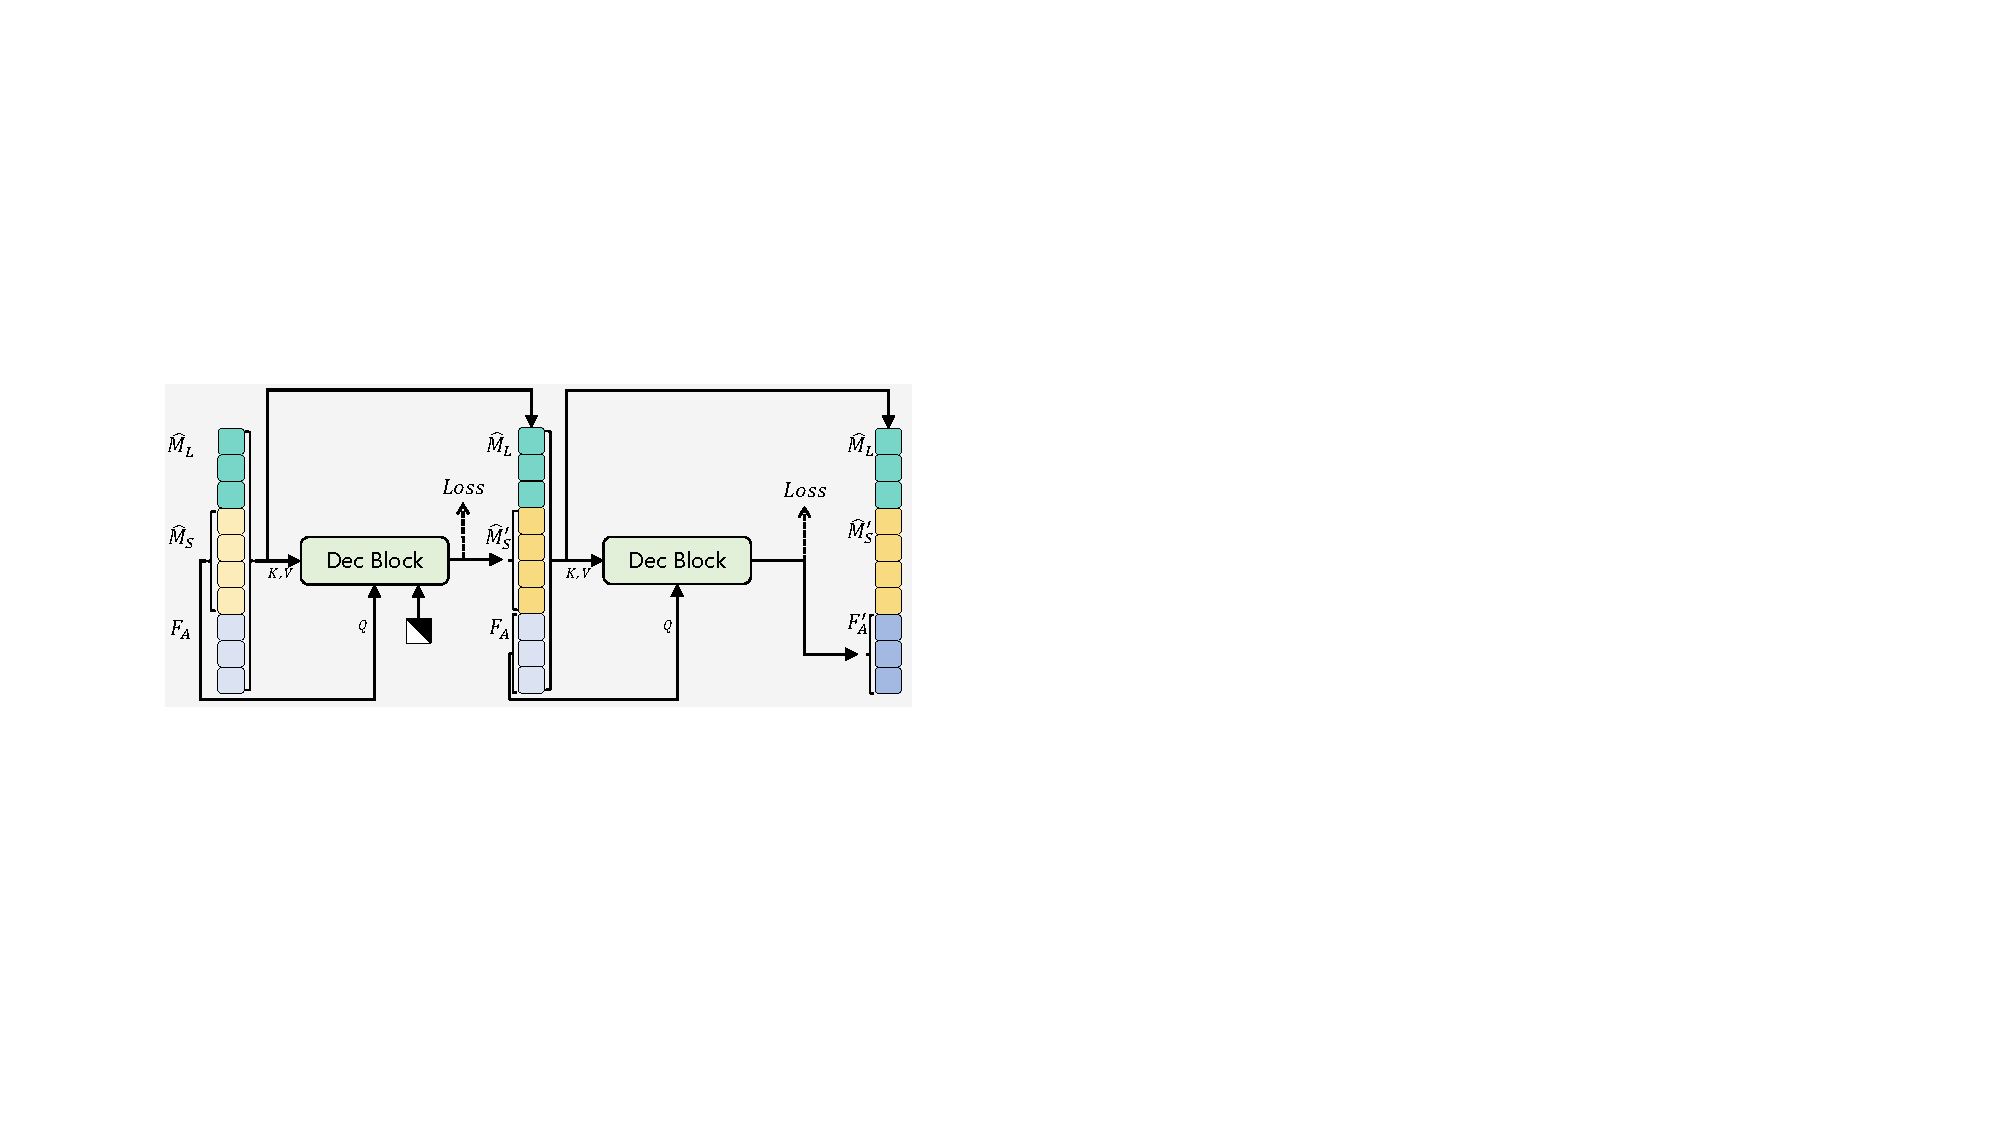
\includegraphics[width=0.48\textwidth]{images/Decoder.pdf}
    \caption{\textbf{Conditional circular interaction} dynamically updates and re-constructs the context between memories and anticipation by aggregating different temporal information. }
    \label{cci}
\end{figure}



\subsection{Training}
\label{training}
Our MAT model relies on action steps of short-term memory to predict the current or future action. 
These steps are utilized as auxiliary information to benefit action detection and anticipation. 
It is worth noting that since the MAT model regards online action detection and anticipation as the same tasks with different settings, we can define the loss function in a unified fashion.

For the  $\mathbf{\widehat{M}}_S$ generated by the encoder, we feed it to a classifier to generate the action probabilities $ \mathbf{\widehat{Y}}_S = \{ \mathbf{\widehat{y}}_S^{i} \}_{i=1}^{m_S} $. 
We then supervise the whole short-term memory using a cross-entropy loss with the labeled action, $ \{ c_S^{i} \}_{i=1}^{m_S} $. 
Learned future features $ \mathbf{F}_A $ are fed into the same classifier to generate the probabilities $ \mathbf{\widehat{Y}}_F = \{ \mathbf{\widehat{y}}_F^{i} \}_{i=1}^{N_F} $ and we also adopt a cross-entropy loss with the target, $ \{ c_F^{i} \}_{i=1}^{m_S} $:
\begin{equation}
    \begin{aligned}
        \mathcal{L}_S^{0}  = -\sum_{i=1}^{m_S}\log\mathbf{\widehat{y}}_S^{i}[c_S^i],
        \mathcal{L}_F^{0}  = -\sum_{i=1}^{N_F}\log\mathbf{\widehat{y}}_F^{i}[c_F^{i}],
    \end{aligned}
\end{equation}
where $\mathcal{L}_S^{0}$ and $\mathcal{L}_F^{0}$ are the loss function of encoded short-term memory and initial anticipation features, respectively.
% For $ \mathbf{\widehat{M}}_S^{\prime} $ and $ \mathbf{F}_A^{\prime} $ obtained from the decoder, we plug same classifier $ \theta $  and $ \theta^{\prime} $to get the classify probabilities. 
As the conditional circular interaction is conducted $ N_t $ times, we use $\mathcal{L}_S^{i}$ and $\mathcal{L}_F^{i}$ to represent the loss of memory and anticipation in each interaction process, where $1 \leq i \leq N_t$. Their calculation is similar to $\mathcal{L}_S^{0}$ and $\mathcal{L}_F^{0}$.
The final training loss is formulated by:
\begin{equation}
    \begin{aligned}
        \mathbf{\mathcal{L}}=\sum_{i=0}^{N_t}\lambda_{s}^{i}\cdot\mathcal{L}_S^{i}+\lambda_f\sum_{i=0}^{N_t}\mathcal{L}_F^{i},
        % \mathbf{\mathcal{L}}_{S}  = \sum_{i=0}^{N_t}\lambda_{i}\cdot\mathcal{L}_S^{i},
        % \mathbf{\mathcal{L}}_{F}  = \sum_{i=0}^{N_t}\mathcal{L}_F^{i},
    \end{aligned}
\end{equation}
where $ \lambda_s^i $ and $ \lambda_f $ are the balance coefficients.





\begin{table*}[t]
    \centering
    \small
    % subfloat
    
    \subfloat[\textbf{Segment number.}\label{tab:segment}]{
    \setlength{\tabcolsep}{2mm}{
    \begin{tabular}[t]{cc}
    % \toprule
        $ N_s $ & mAP \\
        \midrule
        ~\cite{lstr}& 69.6 \\
        2 &  69.8 \\
        4 & 70.2 \\
        \rowcolor{light}
        8 & \textbf{70.4} \\
        12 &  70.1 \\
    % \bottomrule
    \end{tabular}}}
    %}
    %}
    \hspace{1.5mm}
    % subfloat
    \subfloat[\textbf{Future queries renewing.}\label{tab:renew}]{
    % \tablestyle{4pt}{1.05}
    % \footnotesize
    \setlength{\tabcolsep}{2mm}{
    \begin{tabular}[t]{ccc}
    renewal & mAP \\
    \midrule
    0 &  70.0 \\
    \rowcolor{light}
    1 & \textbf{70.4}\\
    2 & 69.7\\
    \\
    \\
    \end{tabular}}}
    \hspace{1.5mm}
    \subfloat[\textbf{Future supervision.}\label{tab:future supervision}]{
    % \tablestyle{4pt}{1.05}
    % \footnotesize
    \setlength{\tabcolsep}{1.5mm}{
    \begin{tabular}[t]{ccc}
    % \toprule
        deep & supervision & mAP \\
         \midrule
         - & cls & 69.9 \\
         \checkmark & feat & 69.6 \\
         \rowcolor{light}
         \checkmark  & cls & \textbf{70.4} \\
         \checkmark  & feat + cls &  70.2 \\
    % \bottomrule
    \\
    \end{tabular}}}
    \hspace{1.5mm}
    \subfloat[\textbf{Shared classifier.}\label{tab:classifier}]{
    % \tablestyle{4pt}{1.05}
    % \footnotesize
    \setlength{\tabcolsep}{1.5mm}{
    \begin{tabular}[t]{ccc}
    % \toprule
        short & future & mAP \\
         \midrule
         % shared &  & 70.0 \\
          % & shared & 69.7 \\
          \multicolumn{2}{c}{unshared} & 69.6 \\
          \multicolumn{2}{c}{separately shared} & 70.1 \\
         % shared & shared & 70.1\\
         \rowcolor{light}
          \multicolumn{2}{c}{full shared} & \textbf{70.4}\\
          \\
         
    % \bottomrule
    \\
    \end{tabular}}}
    \hspace{1.5mm}
    \subfloat[\textbf{MixClip+.}\label{tab:mc+}]{
    \setlength{\tabcolsep}{1mm}{
    \begin{tabular}[t]{llccc}
    % \toprule
        long & short  & V & N & A  \\
        \midrule 
        - & - & 32.1 & 36.1 & 18.1 \\
        MC & - & 32.9 & 36.9 & 18.4 \\
        MC & MC & 31.0 & 37.4 & 18.5 \\
        \rowcolor{light}
        MC & MC+ & \textbf{35.0} & \textbf{38.8} & \textbf{19.5}\\
        MC+ & MC+ & 31.6 & 36.8 & 18.4 \\
    % \bottomrule
    \end{tabular}}}
    \caption{\textbf{Ablation Experiments.} We conduct detailed ablation on (a): Segment number, (b): Future queries renewing, (c): Future supervision, (d): Shared classifier, and (e): MixClip+. The \sethlcolor{light}\hl{gray rows} denote default choices.}
\end{table*}

\subsection{Online Inference}
The existing works~\cite{trn, colar, lstr, testra, avt} test each task independently. 
Thanks to the design of the unified framework, MAT simultaneously infers online action detection and anticipation tasks on one streaming video. It uses the output  $\mathbf{\widehat{M}}_S$ and $ \mathbf{F}_A$ produced by the last interaction as results of online action detection and anticipation, respectively. We take out the last token of $\mathbf{\widehat{M}}_S$ for online action detection. For action anticipation, according to gap time $ \tau$, we take out the corresponding token from $ \mathbf{F}_A$ for forecasting.

